% Compile with XeLaTeX (Liberation Sans = metric-compatible Arial substitute).
\documentclass[aspectratio=169,11pt]{beamer}
\usefonttheme{professionalfonts}
\usepackage[no-math]{fontspec}
\setmainfont{Liberation Sans}
\setsansfont{Liberation Sans}
\usepackage{amsmath,amssymb,bm}
\usepackage{tikz}
\usetikzlibrary{arrows.meta,calc}
\usepackage{booktabs}

% ---------- palette ----------
\definecolor{uoft}{HTML}{1E3765}
\definecolor{ink}{HTML}{1F2933}
\definecolor{muted}{HTML}{66707C}
\definecolor{boxline}{HTML}{8A8A8A}
\definecolor{soft}{HTML}{EEF2F7}
\definecolor{fi}{HTML}{D9822B}   % feature i (frame t1)
\definecolor{fj}{HTML}{C23B3B}   % feature j (frame t2)
\definecolor{good}{HTML}{1E7F6D}
\definecolor{bad}{HTML}{A23B3B}

\newcommand{\iI}{\color{fi}{\bm{i}}}
\newcommand{\jJ}{\color{fj}{\bm{j}}}

\setbeamertemplate{navigation symbols}{}
\hyphenpenalty=10000 \exhyphenpenalty=10000
\setbeamercolor{normal text}{fg=ink}
\setbeamertemplate{itemize item}{-}
\setbeamertemplate{itemize subitem}{\color{muted}--}

% ---------- layout (page is 16 cm x 9 cm) ----------
% Title at top-left, grey content box, UofT logo at bottom-right.
\newcommand{\slidebase}[1]{%
  \node[anchor=base west,text=uoft,font=\fontsize{17}{20}\selectfont] at (0.9,7.8) {#1};
  \node[anchor=south east,inner sep=0] at (15.45,0.3) {
\includegraphics[height=1.05cm]{figures/uoft_logo.png}};
}
\newcommand{\Slide}[2]{%
  \begin{frame}[plain]
  \begin{tikzpicture}[remember picture,overlay,shift={(current page.south west)},x=1cm,y=1cm]
  \slidebase{#1}#2
  \end{tikzpicture}
  \end{frame}}
\newcommand{\keybox}[2]{%
  \node[fill=soft,rounded corners=3pt,inner sep=6pt,text width=#1cm,align=center] {#2};}

\begin{document}

% =========================================================
\begin{frame}[plain]
\begin{tikzpicture}[remember picture,overlay,shift={(current page.south west)},x=1cm,y=1cm]
  \node[anchor=south west,text=uoft,font=\fontsize{22}{27}\selectfont,text width=14cm,align=left] at (0.9,4.75)
    {Coherent Fusion of LiDAR Geometry\\and LiDAR Intensity Images};
  \node[anchor=north west,text=muted,font=\large] at (0.9,4.5) {Uncertainty propagation for intensity-image feature residuals};
  \draw[uoft,line width=1.2pt] (0.9,3.55) -- (4.2,3.55);
  \node[anchor=north west,font=\normalsize] at (0.9,3.3) {Wenda Zhao};
  \node[anchor=south east,inner sep=0] at (15.45,0.3) {
\includegraphics[height=1.05cm]{figures/uoft_logo.png}};
\end{tikzpicture}
\end{frame}

% =========================================================
\Slide{LiDAR--Camera Fusion: Two Different Scales}{
  \node[anchor=north west,inner sep=0] (cl) at (1.15,7.0) {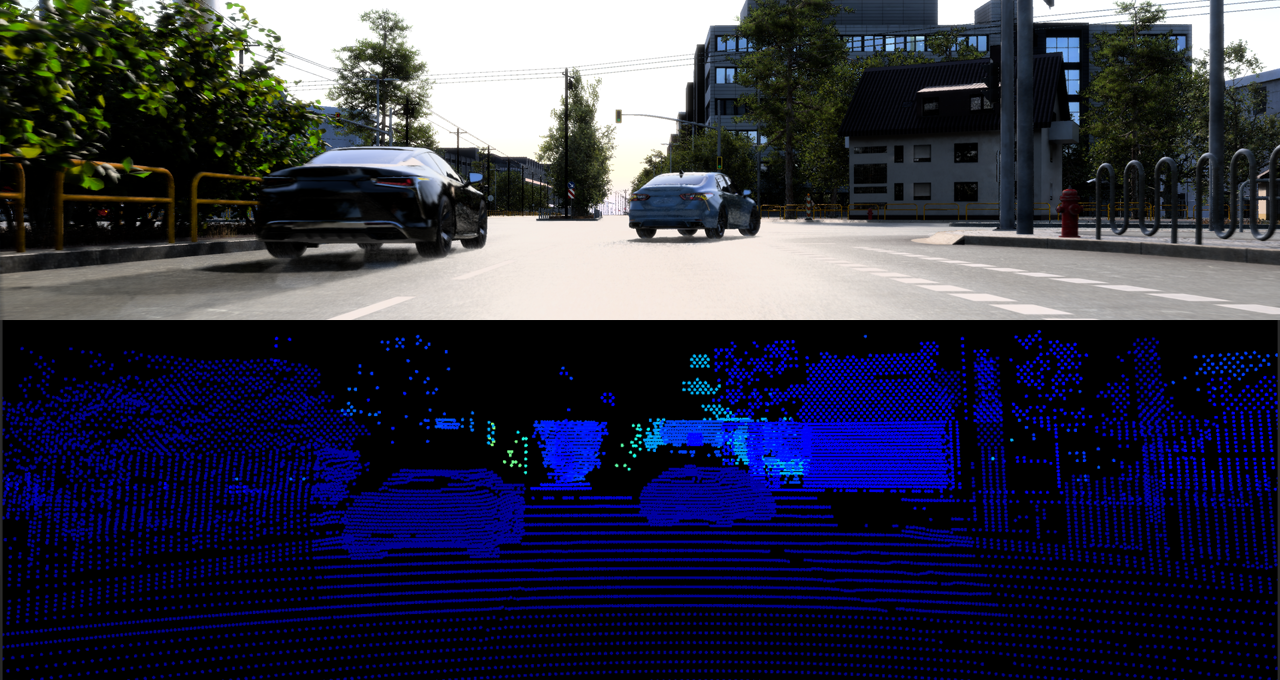
\includegraphics[height=4.4cm]{figures/cam_lidar.png}};
  \node[anchor=north west,font=\small,fill=white,fill opacity=0.85,text opacity=1,inner sep=2pt] at ($(cl.north west)+(0.1,-0.1)$) {\textbf{Camera}: pixels, bearing only};
  \node[anchor=north west,font=\small,fill=white,fill opacity=0.85,text opacity=1,inner sep=2pt] at ($(cl.west)+(0.1,-0.1)$) {\textbf{LiDAR}: meters, bearing + range};
  \node[anchor=north west,font=\normalsize\bfseries,text=uoft] at (9.85,7.0) {1 pixel of error = ? meters};
  \begin{scope}[shift={(9.95,5.55)}]
    \fill[uoft] (0,0) circle (2pt);
    \fill[fi,opacity=0.18] (0,0) -- (4.7,0.6) -- (4.7,-0.6) -- cycle;
    \draw[fi,line width=0.6pt] (0,0) -- (4.7,0.6);
    \draw[fi,line width=0.6pt] (0,0) -- (4.7,-0.6);
    \draw[fj,line width=1.4pt] (1.2,-0.15) -- (1.2,0.15);
    \draw[fj,line width=1.4pt] (4.5,-0.57) -- (4.5,0.57);
    \node[font=\scriptsize,below] at (1.2,-0.2) {near: mm};
    \node[font=\scriptsize,below] at (4.3,-0.62) {far: cm};
  \end{scope}
  \node[anchor=north west,font=\small,align=left] at (9.85,4.3) {%
    -\ \ Depends on \textbf{unknown depth}\\[4pt]
    -\ \ Plus extrinsic, time-sync errors};
  \node[anchor=north west,font=\normalsize\bfseries,text=bad] at (9.85,2.75) {$\Rightarrow$ Weights are tuned by hand};
}

% =========================================================
% VIDEO SLIDE: the poster occupies x = 1.10..10.20 cm, top y = 7.00 cm,
% height = 9.10 * 1168/2524 = 4.21 cm (in the .pptx the video is placed here).
\Slide{Key Insight: The Intensity Image Is the LiDAR Scan}{
  \node[anchor=north west,inner sep=0] (vid) at (1.10,7.0) {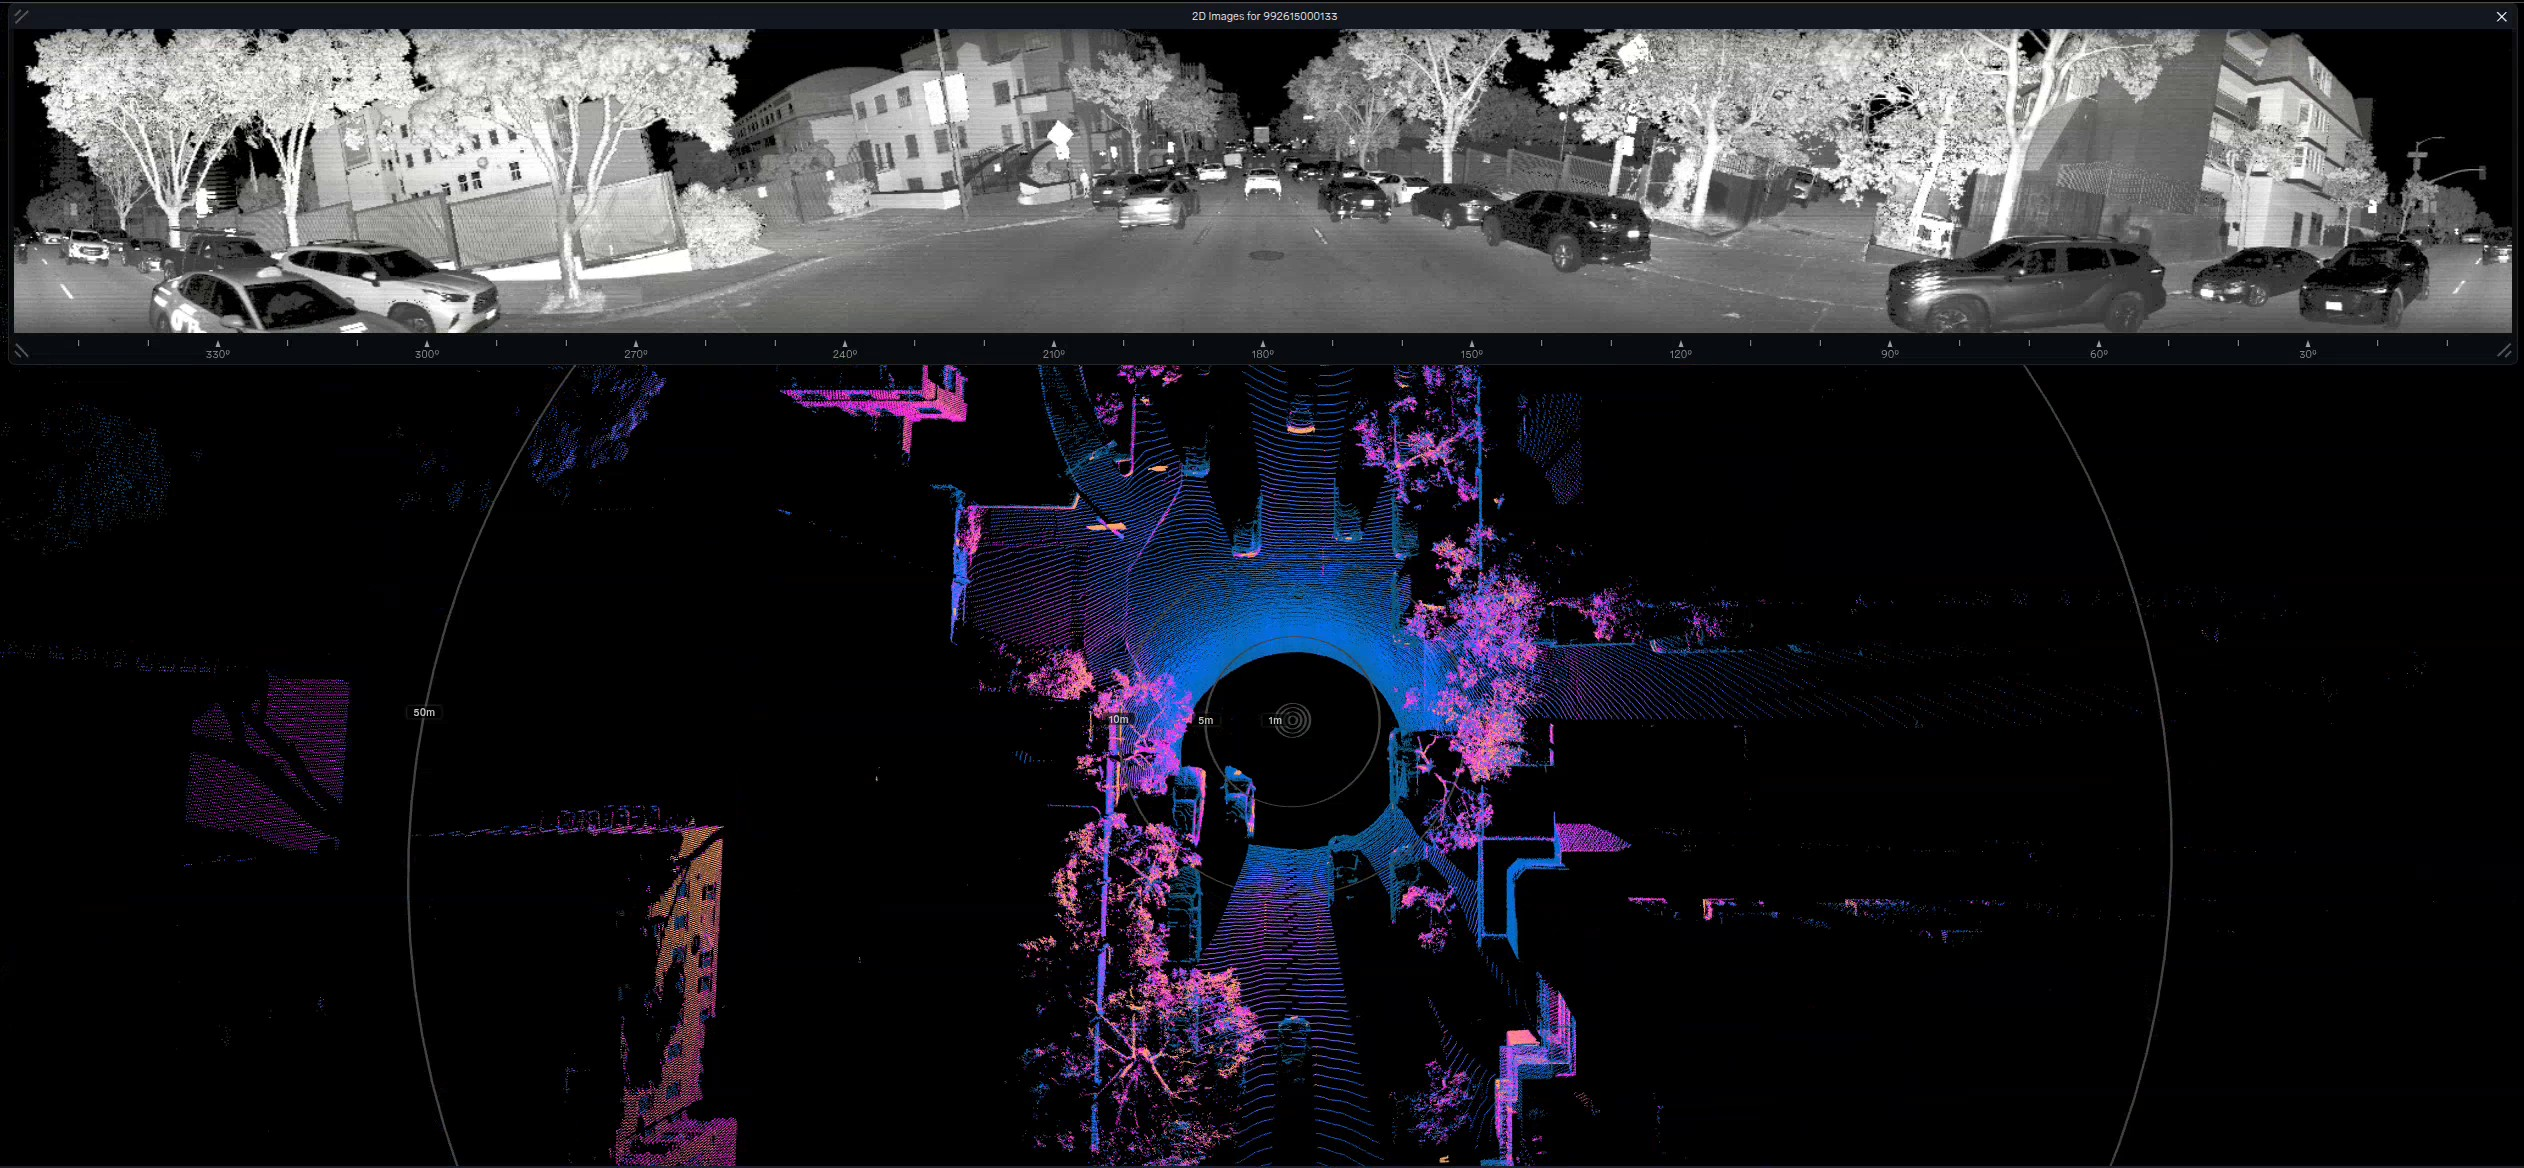
\includegraphics[width=9.1cm]{figures/video_poster.jpg}};
  \node[circle,fill=white,fill opacity=0.85,minimum size=1.1cm] at (vid.center) {};
  \fill[uoft] ($(vid.center)+(-0.17,0.27)$) -- ($(vid.center)+(-0.17,-0.27)$) -- ($(vid.center)+(0.3,0)$) -- cycle;
  \node[anchor=north west,font=\scriptsize,text=muted] at (1.10,2.68) {Top: intensity image. Bottom: point cloud. Same scan, same sensor.};
  \node[anchor=north west,text width=4.95cm,font=\small] at (10.5,7.0) {%
    Each pixel $(u, v)$ also has a \textbf{range} $\rho$:
    \[ \mathbf{z} = \begin{bmatrix} u \\ v \\ \rho \end{bmatrix} \;\leftrightarrow\; \mathbf{p} = f^{-1}(\mathbf{z}) \]
    {\footnotesize\color{uoft}\textbf{One feature = one LiDAR point}}\\[0.4em]
    {\footnotesize\color{muted}Same sensor, same noise model.}};
}

% =========================================================
\Slide{Back-Projecting a Feature to 3D}{
  \node[anchor=north west,text width=7.6cm,font=\normalsize] at (1.15,6.95) {%
    Image coordinates and range of feature $\iI$:
    \[
      \mathbf{z}_{\iI} = \begin{bmatrix} u_{\iI} \\ v_{\iI} \\ \rho_{\iI} \end{bmatrix},\qquad
      \bm{\Sigma}_{\mathbf{z}_{\iI}} = \begin{bmatrix} \bm{\Sigma}_{uv,\iI} & \mathbf{0} \\ \mathbf{0}^{\top} & \sigma_{\rho,\iI}^2 \end{bmatrix}
    \]
    Back-project:};
  \node[anchor=north west] at (1.15,3.95) {\tikz\keybox{8.1}{$\displaystyle \mathbf{p}_{\iI} = f^{-1}(\mathbf{z}_{\iI}), \qquad \bm{\Sigma}_{\mathbf{p}_{\iI}} = \mathbf{J}_{f^{-1},\iI}\,\bm{\Sigma}_{\mathbf{z}_{\iI}}\,\mathbf{J}_{f^{-1},\iI}^{\top}$};};
  \node[anchor=north west,font=\small,text=muted,text width=8.3cm] at (1.15,2.7) {$\mathbf{J}_{f^{-1},\iI} = \partial f^{-1}/\partial\mathbf{z}_{\iI}$; \ $\bm{\Sigma}_{uv}$: learnt; \ $\sigma_\rho^2$: range noise};
  % ellipse figure
  \begin{scope}[shift={(9.6,4.6)},scale=1.1]
    \fill[uoft] (0,0) circle (2.5pt);
    \node[font=\scriptsize,text=muted,below] at (0,-0.1) {LiDAR};
    \draw[muted,dashed] (0,0) -- (4.8,0.58);
    \foreach \r/\w in {1.4/0.2, 2.9/0.42, 4.4/0.65}{
      \begin{scope}[rotate=6.8]
        \fill[fi,opacity=0.25] (\r,0) ellipse (0.13 and \w);
        \draw[fi,line width=0.8pt] (\r,0) ellipse (0.13 and \w);
        \fill[fi] (\r,0) circle (1.3pt);
      \end{scope}
    }
    \draw[-{Stealth[length=2mm]},muted] (0,-1.2) -- (4.8,-1.2) node[midway,below,font=\scriptsize] {range $\rho$};
  \end{scope}
  \node[font=\small,align=center] at (12.25,2.35) {Across the beam: grows with range.\\Along the beam: set by $\sigma_\rho$.};
}

% =========================================================
\Slide{Residual 1: 2D Intensity-Image Feature Residual}{
  \node[anchor=north west,inner sep=0] (m) at (1.15,7.0) {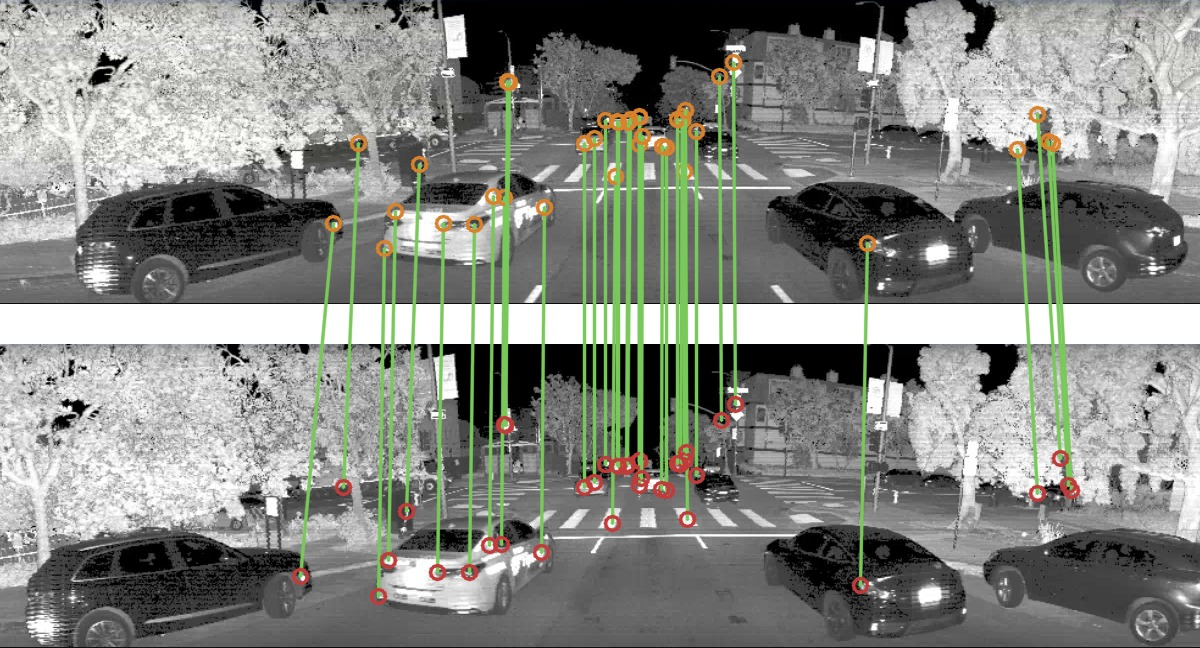
\includegraphics[width=6.0cm]{figures/intensity_matches.jpg}};
  \node[anchor=north,font=\scriptsize,text=muted] at (m.south) [yshift=-0.1cm] {Matched features: {\color{fi}$\iI$ at $t_1$}, {\color{fj}$\jJ$ at $t_2$}};
  \node[anchor=north west,text width=7.2cm,font=\normalsize] at (7.6,7.0) {%
    Lift $\iI$ to 3D, move it to $t_2$, reproject:
    \[
      \hat{\mathbf{p}}_{\jJ} = \mathbf{R}\,\mathbf{p}_{\iI} + \mathbf{t}, \qquad
      \mathbf{r}_{\iI\jJ} = \mathbf{y}_{\jJ} - f(\hat{\mathbf{p}}_{\jJ}) \in \mathbb{R}^2
    \]
    {\small\color{muted} $\mathbf{y}_{\jJ} = [u_{\jJ}, v_{\jJ}]^{\top}$, \quad $\mathbf{J}_{f,\jJ} = \partial f/\partial\hat{\mathbf{p}}_{\jJ}$}};
  \node[anchor=north west] at (1.15,3.0) {\tikz\keybox{13.3}{$\displaystyle
    \bm{\Sigma}_{\mathbf{r}_{\iI\jJ}} =
    \underbrace{\bm{\Sigma}_{uv,\jJ}}_{\text{observed } \jJ}
    + \underbrace{\mathbf{J}_{f,\jJ}\mathbf{R}\,\mathbf{J}_{f^{-1},\iI}\,\bm{\Sigma}_{\mathbf{z}_{\iI}}\,\mathbf{J}_{f^{-1},\iI}^{\top}\mathbf{R}^{\top}\mathbf{J}_{f,\jJ}^{\top}}_{\text{predicted from } \iI}
    + \underbrace{\bm{\Sigma}_{\iI\jJ}^{\mathrm{corr}}}_{\text{matching}}$};};
}

% =========================================================
\Slide{Residual 2: 3D Point-to-Point Feature Residual}{
  % geometry figure
  \begin{scope}[shift={(1.5,3.55)}]
    \fill[uoft] (0,0) circle (2.5pt) node[below,font=\scriptsize,text=muted] {LiDAR at $t_2$};
    \draw[muted,dashed] (0,0) -- (4.4,2.9);
    \draw[muted,dashed] (0,0) -- (5.4,1.9);
    \begin{scope}[shift={(3.9,2.57)},rotate=33.4]
      \fill[fi,opacity=0.22] (0,0) ellipse (0.15 and 0.5);
      \draw[fi,line width=0.8pt] (0,0) ellipse (0.15 and 0.5);
    \end{scope}
    \begin{scope}[shift={(4.8,1.69)},rotate=19.4]
      \fill[fj,opacity=0.22] (0,0) ellipse (0.15 and 0.55);
      \draw[fj,line width=0.8pt] (0,0) ellipse (0.15 and 0.55);
    \end{scope}
    \fill[fi] (3.9,2.57) circle (2pt);
    \node[fi,font=\small,left] at (3.6,2.75) {$\hat{\mathbf{p}}_{\jJ}$};
    \fill[fj] (4.8,1.69) circle (2pt);
    \node[fj,font=\small,right] at (5.05,1.5) {$\mathbf{p}_{\jJ}$};
    \draw[good,line width=1.2pt,-{Stealth[length=2.2mm]}] (3.9,2.57) -- (4.8,1.69);
    \node[good,font=\small,right] at (4.45,2.35) {$\tilde{\mathbf{r}}_{\iI\jJ}$};
  \end{scope}
  \node[anchor=north west,text width=6.9cm,font=\normalsize] at (7.9,7.0) {%
    The match $\jJ$ has a range too, so lift it:
    \[
      \tilde{\mathbf{r}}_{\iI\jJ} = f^{-1}(\mathbf{z}_{\jJ}) - \hat{\mathbf{p}}_{\jJ} \in \mathbb{R}^3
    \]
    {\small Each feature is a \textbf{3D point with a descriptor}: matches give point-to-point pairs without nearest-neighbour search.}};
  \node[anchor=north west] at (1.15,3.0) {\tikz\keybox{13.3}{$\displaystyle
    \bm{\Sigma}_{\tilde{\mathbf{r}}_{\iI\jJ}} =
    \underbrace{\mathbf{J}_{f^{-1},\jJ}\,\bm{\Sigma}_{\mathbf{z}_{\jJ}}\,\mathbf{J}_{f^{-1},\jJ}^{\top}}_{\text{observed } \jJ}
    + \underbrace{\mathbf{R}\,\mathbf{J}_{f^{-1},\iI}\,\bm{\Sigma}_{\mathbf{z}_{\iI}}\,\mathbf{J}_{f^{-1},\iI}^{\top}\mathbf{R}^{\top}}_{\text{predicted from } \iI}
    + \underbrace{\bm{\Sigma}_{\iI\jJ}^{\mathrm{corr}}}_{\text{matching}}$};};
}

% =========================================================
\Slide{Two Residuals, One Noise Model}{
  \node[anchor=north,font=\small] at (7.97,6.95) {%
    \renewcommand{\arraystretch}{1.45}
    \begin{tabular}{p{3.0cm}p{4.6cm}p{4.6cm}}
      \toprule
      & \textbf{2D feature residual} & \textbf{3D point-to-point residual} \\
      \midrule
      Residual & $\mathbf{y}_{\jJ} - f(\hat{\mathbf{p}}_{\jJ})$ \; (pixels) & $f^{-1}(\mathbf{z}_{\jJ}) - \hat{\mathbf{p}}_{\jJ}$ \; (meters) \\
      Range used & frame $t_1$ & frames $t_1$ and $t_2$ \\
      Pose Jacobian & $-\mathbf{J}_{f,\jJ}\,\partial\hat{\mathbf{p}}_{\jJ}/\partial\bm{\xi}$ & $-\partial\hat{\mathbf{p}}_{\jJ}/\partial\bm{\xi}$ \;(as in ICP) \\
      Observed side & $\bm{\Sigma}_{uv,\jJ}$ & $\mathbf{J}_{f^{-1},\jJ}\bm{\Sigma}_{\mathbf{z}_{\jJ}}\mathbf{J}_{f^{-1},\jJ}^{\top}$ \\
      \bottomrule
    \end{tabular}};
  \node[anchor=north] at (7.97,3.3) {\tikz\keybox{13.6}{\normalsize Both are built from the same $\bm{\Sigma}_{\mathbf{p}} = \mathbf{J}_{f^{-1}}\bm{\Sigma}_{\mathbf{z}}\mathbf{J}_{f^{-1}}^{\top}$ and the same LiDAR noise.};};
}

% =========================================================
\Slide{Coherent Fusion without Hand-Tuned Weights}{
  \node[anchor=north west,text width=6.3cm] at (1.15,7.0) {%
    {\color{bad}\textbf{LiDAR + camera}}
    \begin{itemize}\small\setlength{\itemsep}{2pt}
      \item Two sensors, two noise models
      \item Pixel-to-meter scale is unknown
      \item Relative weight tuned until it works
    \end{itemize}};
  \node[anchor=north west,text width=6.6cm] at (8.2,7.0) {%
    {\color{good}\textbf{LiDAR + intensity image}}
    \begin{itemize}\small\setlength{\itemsep}{2pt}
      \item One sensor: one feature = one point
      \item Every residual covariance is propagated from $\bm{\Sigma}_{uv}$ and $\sigma_\rho^2$
      \item Weights follow from the noise model
    \end{itemize}};
  \draw[boxline!60] (7.95,6.9) -- (7.95,4.6);
  \node[anchor=north] at (7.97,4.2) {\tikz\keybox{11}{%
    $\displaystyle \bigl(\mathbf{H}_g + \mathbf{P}_d\mathbf{H}_I\mathbf{P}_d\bigr)\,\delta\mathbf{x} = \mathbf{b}_g + \mathbf{P}_d\mathbf{b}_I,
    \qquad \mathbf{H}_I = \sum \mathbf{J}_{\xi}^{\top}\bm{\Sigma}_{\mathbf{r}}^{-1}\mathbf{J}_{\xi}$\\[4pt]
    {\small\color{muted} $\mathbf{P}_d$: projector onto the geometrically degenerate directions}};};
}

% =========================================================
\Slide{Takeaways}{
  \node[anchor=north west,text width=13.2cm,font=\normalsize] at (1.15,6.9) {%
    \begin{itemize}\setlength{\itemsep}{10pt}
      \item \textbf{Gap:} LiDAR--camera fusion has no common scale, so weights are hand-tuned.
      \item \textbf{Insight:} in a LiDAR intensity image, one feature is one LiDAR point.
      \item \textbf{Derivation:} propagate $\bm{\Sigma}_{\mathbf{z}} = \mathrm{diag}(\bm{\Sigma}_{uv}, \sigma_\rho^2)$ into a 2D feature residual and a 3D point-to-point residual.
      \item \textbf{Result:} LiDAR geometry and intensity features fuse coherently, with no tuned weight.
    \end{itemize}};
}

\end{document}
